% Created 2015-02-02 Mon 09:16
\documentclass[a4paper]{article}
\usepackage[utf8]{inputenc}
\usepackage[T1]{fontenc}
\usepackage{fixltx2e}
\usepackage{graphicx}
\usepackage{longtable}
\usepackage{float}
\usepackage{wrapfig}
\usepackage{rotating}
\usepackage[normalem]{ulem}
\usepackage{amsmath}
\usepackage{textcomp}
\usepackage{marvosym}
\usepackage{wasysym}
\usepackage{amssymb}
\usepackage{hyperref}
\tolerance=1000
\setlength\parindent{0pt}
\usepackage{titling}
\addtolength{\topmargin}{-1.375in}
\addtolength{\textheight}{1.75in}
\addtolength{\oddsidemargin}{-.375in}
\addtolength{\evensidemargin}{-.875in}
\addtolength{\textwidth}{0.75in}
\author{Michael Hunsinger}
\date{\today}
\title{Assignment One}
\hypersetup{
  pdfkeywords={},
  pdfsubject={},
  pdfcreator={Emacs 24.4.1 (Org mode 8.2.10)}}
\begin{document}

\maketitle

\section*{Question One}
\label{sec-1}
Below is a ``smart'' search tree for the game provided. \\

\begin{center}
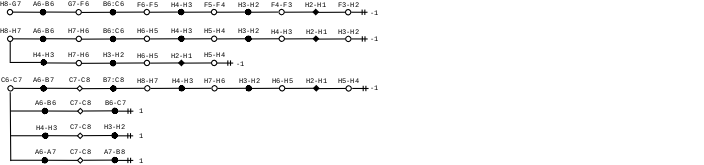
\includegraphics[width=.9\linewidth]{./multimedia/search-tree.png}
\end{center}

The ``smart'' search tree was contstructed with the following assumption in
mind: The game is over if the target is destroyed and the piece could not
be caputered by the opponenent on the next turn (the following opponents move
was shown to illustrate this). If a move destroyed the target, it is denoted 
on the tree with a diamond rather than a circle. \\

This tree is very condensed from the full search tree and even a full ``smart''
search. However, the tree does illustrate the edge cases and the reader can
draw conclusions from those to see that any case inbetween will result in the
same outcome. \\

For instance, if the black King persues the white pawn, and the white King
moves diagonally, to try and support the pawn, it does not make it in time
(first branch). It also shows that if the white King directly persues the
black Pawn, the black King can capture the white Pawn and still leave time for
the black Pawn to advance and destroy the target before the white King can
intercept. From this, we can easily infer the white King could advance along
the diagonal, and still fall short of reaching the black Pawn before
it destroys the target (even though the number of moves did not change).

Black appears to have the advantage in this game. The only way white may win
is if it's Pawn persues the target first and the black King does not persue
the Pawn on the diagonal towards the target.

\section*{Question Two}
\label{sec-2}
\subsection*{Part A}
\label{sec-2-1}
The general reachability formula for the Queen is as follows.

\begin{equation}
\begin{split}
R_Q(x, y) = \; &(x = (x_1, x_2) \wedge (1 \leq x_1 \leq 8) 
\wedge (1 \leq x_2 \leq 8)) \;\wedge \\
&(y = (y_1, y_2) \wedge (1 \leq y_1 \leq 8) 
\wedge (1 \leq y_2 \leq 8)) \;\wedge \\
&(|y_1 - x_1| \leq 8 \wedge |y_2 - x_2| \leq 8) \\
\end{split}
\end{equation}

x $\in$ Z \texttimes{} Z, y $\in$ Z \texttimes{} Z

\subsection*{Part B}
\label{sec-2-2}
The reachability formulas for the King in a three dimensional space is as
follows:

\begin{equation}
\begin{split}
R_K(x, y, z) = \; &(x = (x_1, x_2) \wedge (1 \leq x_1 \leq 8) 
                                   \wedge (1 \leq x_2 \leq 8)) \;\wedge \\
                  &(y = (y_1, y_2) \wedge (1 \leq y_1 \leq 8) 
                                   \wedge (1 \leq y_2 \leq 8)) \;\wedge \\
                  &(z = (z_1, z_2) \wedge (1 \leq z_1 \leq 8) 
                                   \wedge (1 \leq z_2 \leq 8)) \;\wedge \\
               &(|y_1 - x_1 - z_1| \leq 1 \wedge |y_2 - x_2 - z_2| \leq 1)\\
\end{split}
\end{equation}

The reachability formulas for the Knight in a three dimensional space is as
follows:

\begin{equation}
\begin{split}
R_K(x, y, z) = \; &(x = (x_1, x_2) \wedge (1 \leq x_1 \leq 8) 
                                   \wedge (1 \leq x_2 \leq 8)) \;\wedge \\
                  &(y = (y_1, y_2) \wedge (1 \leq y_1 \leq 8) 
                                   \wedge (1 \leq y_2 \leq 8)) \;\wedge \\
                  &(z = (z_1, z_2) \wedge (1 \leq z_1 \leq 8) 
                                   \wedge (1 \leq z_2 \leq 8)) \;\wedge \\
               &(|y_1 - x_1 - z_1| = 1 \wedge |y_2 - x_2 - z_2| = 2)\;\vee \\
               &(|y_1 - x_1 - z_1| = 2 \wedge |y_2 - x_2 - z_2| = 1)
\end{split}
\end{equation}

Assuming the following both of the equations:

\begin{equation}
x \in Z \times Z, y \in Z \times Z, z \in Z \times Z
\end{equation}
% Emacs 24.4.1 (Org mode 8.2.10)
\end{document}
